\section{Multi-Agent Stock Analysis Design}
\label{sec:multi-agent-stock-analysis-design}

Stockrium implements stock analysis as a stateful directed graph rather than as one monolithic language-model prompt. The current version separates deterministic planning, source-data preparation, source-specific interpretation, recommendation scoring, trading-plan generation, and final presentation. This separation is important because price series require numerical calculation, annual indicators require multi-year and industry-aware preparation, and articles require semantic interpretation. It also allows automatic and manually configured requests to share one implementation while skipping sources that the manual request does not enable.

LangGraph provides the state-graph abstraction used to declare nodes, conditional edges, shared state, and parallel branches \cite{langgraph2026graphapi}. The graph uses DeepSeek for source interpretation and normalized source scoring, conditional trading-plan generation, and final narrative synthesis. Python retains control over date windows, candle intervals, technical-indicator and trend-feature calculation, deterministic reference signals, weighted recommendation scoring, decision thresholds, and validation of trading-plan constraints. The implementation is therefore hybrid: the model interprets bounded evidence and produces component scores and explanations, while Python deterministically combines the validated scores into the Buy-or-Wait decision.

\subsection{Graph Topology and Shared State}
\label{subsec:analysis-graph-state}

The compiled analysis graph contains nine nodes. The orchestrator first creates a deterministic plan and conditionally activates up to three source branches. Each enabled branch contains a data-preparation node followed by an analysis node: \texttt{article\_agent} feeds \texttt{article\_analysis\_agent}, \texttt{fundamental\_agent} feeds \texttt{fundamental\_analysis\_agent}, and \texttt{technical\_agent} feeds \texttt{technical\_analysis\_agent}. The completed branch scores converge at \texttt{recommendation\_agent}, which makes the deterministic decision and, for a Buy result, constructs a trading plan. The final \texttt{aggregator} generates only confidence and a concise summary before assembling the public response. Figure~\ref{fig:analysis-graph-topology} presents this execution topology.

\begin{figure}[H]
    \centering
    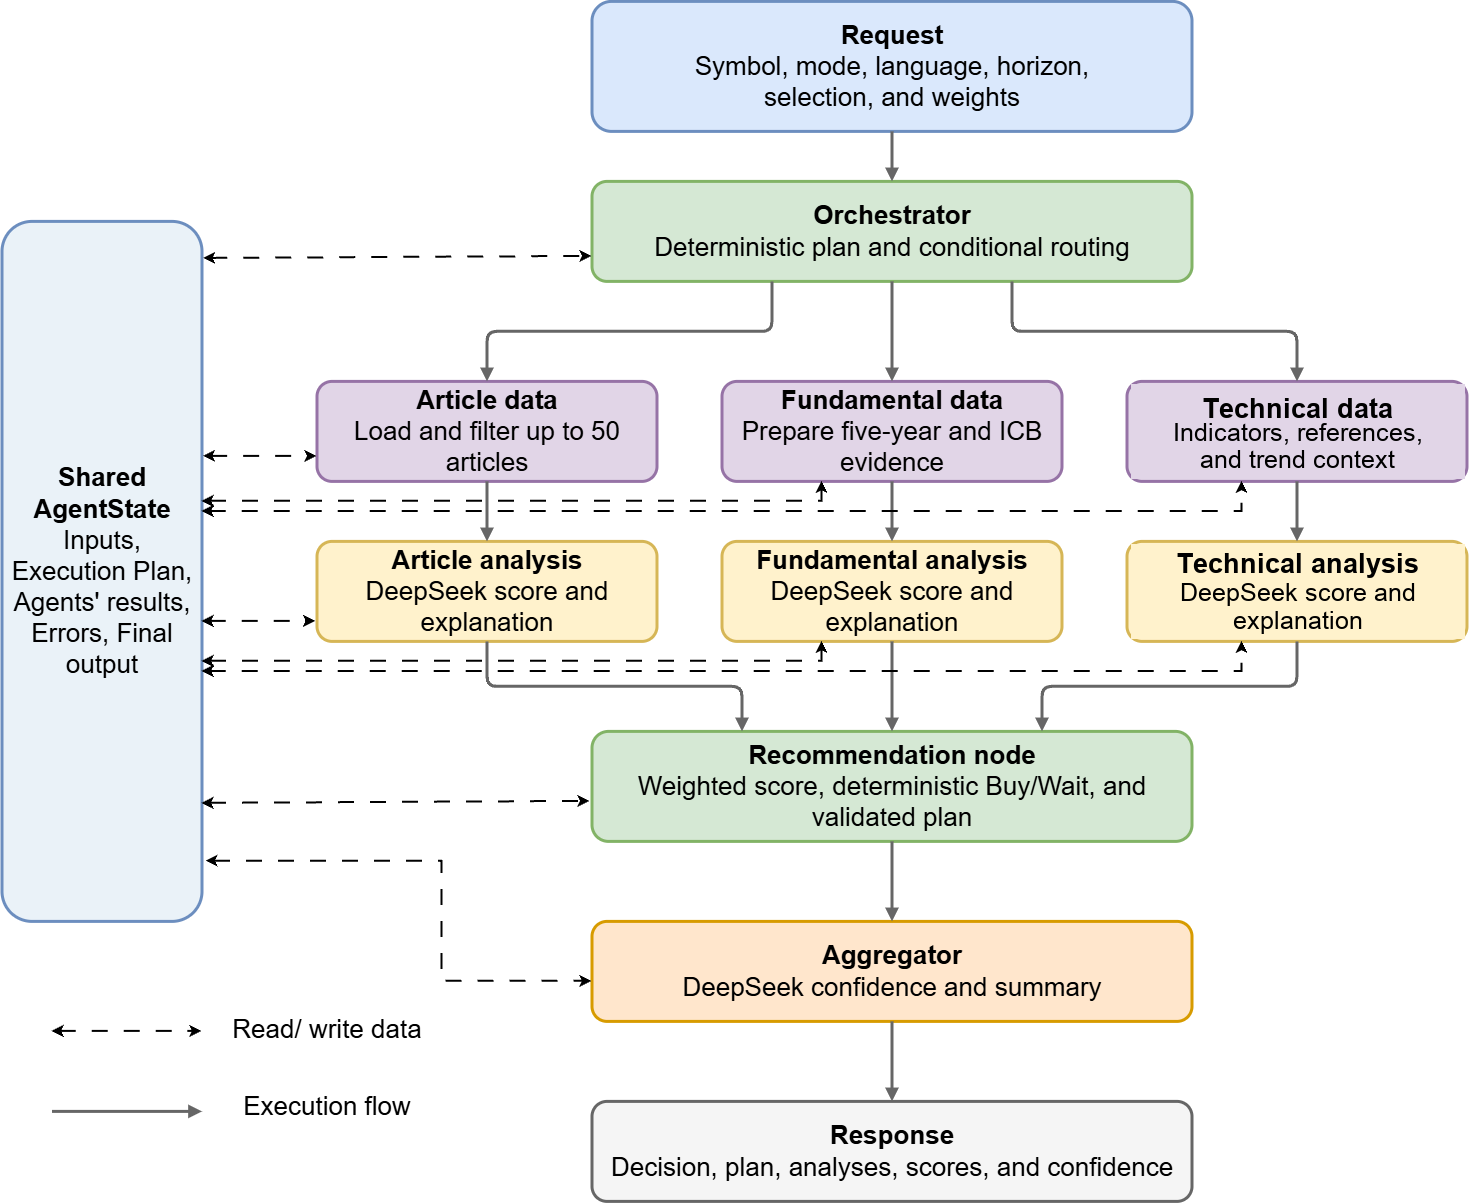
\includegraphics[height=0.6\textheight,keepaspectratio]{figures/chapter4/stockrium_agent_topology_portrait.png}
    \caption{Execution topology of the current Stockrium analysis graph}
    \label{fig:analysis-graph-topology}
\end{figure}

The three source chains can execute in parallel after orchestration. Their updates are written to separate keys in \texttt{agent\_results}, whose \texttt{operator.or\_} reducer merges branch dictionaries instead of allowing the last completed branch to replace earlier results. LangGraph waits at the convergence into \texttt{recommendation\_agent}; recommendation and aggregation then execute sequentially.

The shared \texttt{AgentState} fields are summarized in Table~\ref{tab:analysis-workflow-state}. A node reads the context it requires and returns only the state fields that it changes.

\begin{table}[H]
    \centering
    \caption{Principal fields in the current analysis graph state}
    \label{tab:analysis-workflow-state}
    \small
    \setlength{\tabcolsep}{5pt}
    \renewcommand{\arraystretch}{1.18}
    \begin{tabular}{p{3.0cm} p{3.0cm} p{6.5cm}}
        \toprule
        \textbf{Field} & \textbf{Producer} & \textbf{Purpose} \\
        \midrule
        \texttt{mode} & API service & Selects automatic or manual analysis; \texttt{chat} is permitted by the type contract but the public stock-analysis request accepts only the first two values. \\
        \texttt{language} & API service & Selects Vietnamese or English for user-facing model output and deterministic fallback messages. \\
        \texttt{user\_input} & API service & Localized analysis request retained as request context. \\
        \texttt{risk\_appetite} & API service & Contains \texttt{short\_term}, \texttt{mid\_term}, or \texttt{long\_term}, which controls date windows, interval, default weights, and plan bounds. \\
        \texttt{symbol} & API service & Identifies the listed security being analyzed. \\
        \texttt{data\_selection} & API service & Contains news and fundamental switches, five technical-indicator switches, and optional manual weights. \\
        \texttt{plan} & Orchestrator & Supplies deterministic article and technical date ranges and the technical interval. \\
        \texttt{agent\_results} & Graph nodes & Merge-reduced dictionary containing prepared evidence, source analyses, and the recommendation result. \\
        \texttt{final\_output} & Aggregator & Public structured response returned by the application service. \\
        \texttt{error} & Aggregator or caller & Carries an unrecovered terminal failure to the application service. \\
        \bottomrule
    \end{tabular}
\end{table}

Automatic mode ignores the submitted selection and routes all three source chains. Manual mode routes news only when \texttt{news} is true, routes fundamentals only when \texttt{fundamental} is true, and routes technical analysis when at least one of \texttt{ma}, \texttt{boll}, \texttt{rsi}, \texttt{macd}, or \texttt{kdj} is true. The public request schema requires at least one technical indicator, so a valid public manual request always executes the technical chain. A skipped source does not produce a disabled marker because its nodes are not executed.

\subsection{Deterministic Horizon-Aware Planning}
\label{subsec:analysis-orchestrator-planning}

The orchestrator does not call a language model. It reads \texttt{risk\_appetite.period}, obtains the current date in Vietnam time (UTC+7), and applies the fixed rules in Table~\ref{tab:analysis-plan-rules}. This makes two requests with the same horizon and analysis date use the same evidence windows and technical interval.

\begin{table}[H]
    \centering
    \caption{Deterministic planning rules by investment horizon}
    \label{tab:analysis-plan-rules}
    \small
    \renewcommand{\arraystretch}{1.2}
    \begin{tabular}{lccc}
        \toprule
        \textbf{Horizon} & \textbf{Technical interval} & \textbf{Technical lookback} & \textbf{Article lookback} \\
        \midrule
        Short term & 1 hour & 90 days & 30 days \\
        Medium term & 1 day & 365 days & 90 days \\
        Long term & 1 week & 1,825 days & 365 days \\
        \bottomrule
    \end{tabular}
\end{table}

One-hour candles are aggregated from \texttt{Stock\_Price\_1m}; daily candles are read from \texttt{Stock\_Price\_1d}; and weekly candles are aggregated from the daily table. The plan does not contain a fundamental date range during live analysis because the fundamental node always selects up to the five latest annual indicator rows. The historical backtesting adapter reuses the same agents with a fixed medium-term/daily configuration, sets the requested date as the plan end date, disables \texttt{Current\_Stock\_Price} lookup, and excludes fundamental rows from the simulated year and all future years.

\subsection{Two-Stage Specialist Source Chains}
\label{subsec:analysis-specialist-nodes}

Each specialist branch separates evidence preparation from semantic interpretation. The preparation node reads application services and produces a bounded evidence object or text block. The following analysis node either calculates or generates a normalized score in $[0,1]$ and produces a user-facing explanation. Table~\ref{tab:specialist-node-responsibilities} summarizes the implemented behavior.

\begin{table}[H]
    \centering
    \caption{Implemented specialist source chains}
    \label{tab:specialist-node-responsibilities}
    \footnotesize
    \setlength{\tabcolsep}{4pt}
    \renewcommand{\arraystretch}{1.18}
    \begin{tabular}{p{2.2cm} p{4.3cm} p{4.4cm} p{2.5cm}}
        \toprule
        \textbf{Source} & \textbf{Preparation node} & \textbf{Analysis node} & \textbf{Score origin} \\
        \midrule
        Technical & Loads OHLCV, obtains the current snapshot when permitted, calculates indicators, retains binary reference signals, and constructs a 20-candle trend context for price, volume, and selected indicators. & DeepSeek returns a structured technical \texttt{score} and explanatory \texttt{analysis}; the binary ratio is retained only as an error fallback. & DeepSeek, constrained to $[0,1]$. \\
        Fundamental & Loads annual \texttt{FA\_Indicator} rows, company ICB context, and \texttt{FA\_Industry\_Aggregate}; formats five-year metrics, CAGR, DuPont, and peer comparisons. & DeepSeek returns a structured fundamental \texttt{score} and explanatory \texttt{analysis}. & DeepSeek, constrained to $[0,1]$. \\
        Article & Loads stock-associated articles in the planned dates, sorts newest first, retains at most 50, and formats title, date, summary/description, and stored sentiment. & DeepSeek returns a structured news \texttt{score} and explanatory \texttt{analysis}. & DeepSeek, constrained to $[0,1]$. \\
        \bottomrule
    \end{tabular}
\end{table}

The analysis nodes call the model configured by \texttt{DEEPSEEK\_MODEL}, whose default is \texttt{deepseek-v4-flash}, through DeepSeek's OpenAI-compatible endpoint. They request JSON-object mode, append the target Pydantic JSON Schema to the system prompt, disable thinking mode, and validate the returned JSON with Pydantic. The helper makes at most two attempts when the model returns empty or invalid structured content. Source analysis, trading-plan generation, and aggregation all use temperature 0.1. The selected application language is appended to the calls that generate user-facing explanations, so the same graph can return Vietnamese or English analytical text.

\subsubsection{Technical Source and Analysis Nodes}
\label{subsubsec:technical-analysis-node}

The technical preparation node loads the interval selected by the orchestrator and requires at least 50 valid OHLCV candles before calculating the full indicator frame. For live analysis it attempts to read the latest positive matched value from \texttt{Current\_Stock\_Price}; if no valid snapshot is available, the current-price field falls back to the close of the most recent candle in the requested period. Indicator comparisons always use that candle and its predecessor rather than the separate live snapshot. The historical adapter explicitly disables the snapshot lookup, so its current-price field is the candidate-date candle close.

Each enabled indicator still contributes either zero or one deterministic reference point. The denominator \texttt{max\_score} is the number of selected indicators, so a manual single-indicator request has one reference point rather than five. These values support interpretable reasons, historical candidate prefiltering, single-indicator ablations, and fallback behavior; they are no longer the primary production technical score. Table~\ref{tab:technical-signal-scoring} lists the implemented positive conditions.

\begin{table}[H]
    \centering
    \caption{Deterministic positive-signal conditions in the technical source node}
    \label{tab:technical-signal-scoring}
    \footnotesize
    \setlength{\tabcolsep}{4pt}
    \renewcommand{\arraystretch}{1.18}
    \begin{tabular}{p{1.65cm} p{10.9cm}}
        \toprule
        \textbf{Indicator} & \textbf{One-point conditions evaluated by Python} \\
        \midrule
        RSI & Crosses upward through 50; is between 50 and 70 and rising; or is below 35 but recovering. \\
        Moving averages & SMA20 crosses upward through SMA50; SMA20 is above SMA50 with an expanding gap; or close is above SMA20 while SMA20 is above SMA50. \\
        Bollinger Bands & Close crosses upward through the middle band; remains above the middle band with an expanding distance; or recovers while at or below the lower band. \\
        MACD & MACD crosses upward through its signal line; remains above the signal while the histogram strengthens; or the histogram changes from negative to nonnegative. \\
        KDJ & K recovers while below 20; crosses upward through D; or remains above D while J rises. A current K above 80 is checked first and scores zero. \\
        \bottomrule
    \end{tabular}
\end{table}

For each selected indicator, the source output contains the current and previous values, the binary reference score, and a rule-generated reason. It also contains the requested and actual periods, candle count, interval, source table, current display price, \texttt{total\_score}, and \texttt{max\_score}. In addition, \texttt{trend\_context} uses 21 observations to represent a 20-candle lookback. It supplies 1-, 5-, 10-, and 20-candle returns; the latest close and its position in the observed high--low range; counts of rising, falling, and unchanged closes; current volume, its one-candle change, five- and twenty-candle averages, and current-to-average ratios; one- and five-candle changes plus extrema for every selected indicator field; and the recent OHLCV and indicator sequence. Only the indicators enabled by the request are included, while OHLCV and available volume averages remain available for confirmation.

DeepSeek receives this bounded object and returns the production technical score and explanation together:

\begin{equation}
    (c_t,a_t)=\operatorname{DeepSeek}(E_t),
    \qquad c_t\in[0,1],
    \label{eq:technical-normalized-score}
\end{equation}

where $E_t$ is the prepared technical evidence and $a_t$ is the natural-language analysis. The prompt defines five score bands from strongly bearish ($0.00$--$0.19$) to strongly bullish ($0.80$--$1.00$) and instructs the model to evaluate multi-candle price structure, moving-average direction, MACD momentum, RSI and KDJ context, Bollinger-band position and width, and price--volume confirmation jointly rather than averaging indicator labels. It also distinguishes the live display price used for the trading plan from the candle close used by the indicators because their source units may differ. If structured model analysis fails while source data remain valid, Python falls back to \texttt{total\_score/max\_score}, clamps it to $[0,1]$, and returns a localized failure explanation.

\subsubsection{Fundamental Source and Analysis Nodes}
\label{subsubsec:fundamental-analysis-node}

The fundamental source node reads annual records from \texttt{FA\_Indicator}. It uses \texttt{BI\_Profile.icb\_code} only to identify financial-sector companies and to load the corresponding precomputed industry aggregate. The current node does not load income-statement, cash-flow, balance-sheet, or stored-summary text directly. It sorts valid years, keeps the five latest rows, and presents missing metrics as unavailable rather than inferring them.

For metrics that permit growth calculation, the node uses

\begin{equation}
    \operatorname{CAGR}(x) = \left(\frac{x_n}{x_0}\right)^{\frac{1}{y_n-y_0}} - 1,
    \label{eq:fundamental-cagr}
\end{equation}

where both endpoints must be positive and at least two valid observations with a positive elapsed period must exist \cite{damodaranHistoricalGrowth2026}. For nonfinancial firms, the formatted sections cover liquidity, leverage, operating efficiency, profitability, and valuation. When the necessary fields exist, the source also presents the three-factor DuPont decomposition \cite{openstaxDupont2022}:

\begin{equation}
    ROE = \text{Net Margin} \times \text{Asset Turnover} \times \text{Financial Leverage}.
    \label{eq:dupont-stockrium}
\end{equation}

An ICB code beginning with 8 selects the financial-sector layout: capital safety, asset quality/management, earnings, liquidity, and P/B-based valuation. The industry comparison is emitted only when the maximum reported peer count is at least three. It includes the latest company and industry-median values and their available CAGRs. DeepSeek then converts this prepared evidence into a normalized fundamental score $c_f\in[0,1]$ and an explanation. Missing data or an unrecovered analysis error produces $c_f=0$ with a localized no-data or failure message.

\subsubsection{Article Source and Analysis Nodes}
\label{subsubsec:article-analysis-node}

The article source node retrieves records already associated with the selected symbol, keeps only records whose publication dates fall inside the orchestrator's inclusive range, sorts them from newest to oldest, and retains at most 50. Each prompt entry contains the publication date, title, up to 1,200 characters from the available summary or description, and stored sentiment when present.

DeepSeek is instructed to use only the supplied articles, merge duplicated information, emphasize events that directly affect the company, and return a positivity score $c_n\in[0,1]$ together with a concise explanation of drivers and risks. It does not generate entry or exit prices. When the period contains no article, loading fails, or structured analysis cannot be recovered, the branch returns a zero score and an explicit localized message. In the recommendation formula, this is a zero component rather than a separately renormalized missing source.

\subsection{Deterministic Recommendation and Trading Plan}
\label{subsec:analysis-recommendation-controls}

The recommendation node receives the three normalized component scores. Default weights vary by investment horizon as shown in Table~\ref{tab:confidence-horizon-weights}. The allocation was defined for Stockrium after domain consultation with Ms.~Trinh, Securities Analyst at FPT Securities Joint Stock Company \cite{trinh2026weights}.

\begin{table}[H]
    \centering
    \caption{Default recommendation-score weights by investment horizon, based on expert consultation \protect\cite{trinh2026weights}}
    \label{tab:confidence-horizon-weights}
    \small
    \renewcommand{\arraystretch}{1.2}
    \begin{tabular}{lccc}
        \toprule
        \textbf{Horizon} & \textbf{Technical} & \textbf{Fundamental} & \textbf{News} \\
        \midrule
        Short term & 0.60 & 0.10 & 0.30 \\
        Medium term & 0.40 & 0.40 & 0.20 \\
        Long term & 0.15 & 0.70 & 0.15 \\
        \bottomrule
    \end{tabular}
\end{table}

Manual mode can replace these values with request weights for news, technical, and fundamental evidence. The request schema constrains each value to $[0,1]$, permits at most two decimal places, and requires the three values to total 1.0. The recommendation node checks the total again and falls back to the horizon defaults if called with an invalid internal payload. The implementation does not renormalize weights after a source is disabled or unavailable: an absent branch has score zero. A manual request that intentionally disables a source should therefore assign it zero weight if the remaining sources are intended to carry the complete score.

Let $c_t$, $c_f$, and $c_n$ denote technical, fundamental, and news scores and let the corresponding effective request or horizon weights be $w_t$, $w_f$, and $w_n$. The weighted total uses one common acceptance threshold, while the technical threshold depends on the investment horizon:

\begin{equation}
    \tau_t(h)=
    \begin{cases}
        0.60, & h=\texttt{short\_term},\\
        0.50, & h=\texttt{mid\_term},\\
        0.40, & h=\texttt{long\_term}.
    \end{cases}
\end{equation}

For an automatic request, and for a manual request whose effective technical weight is at least 0.15, the technical gate is active. A valid manual request with $w_t<0.15$ bypasses that gate so that a deliberately de-emphasized technical source cannot veto the other evidence. The implemented decision is therefore

\begin{equation}
    S = w_t c_t + w_f c_f + w_n c_n,
    \qquad
    \textit{Buy} \iff S \geq 0.60
    \;\land\;
    \left(c_t \geq \tau_t(h)\;\lor\;(\texttt{manual}\land w_t<0.15)\right).
    \label{eq:recommendation-score}
\end{equation}

Thus the language model produces the technical, fundamental, and news component scores but does not directly propose Buy or Wait. There are no separate weak-fundamental or negative-news label vetoes in the current code. Python returns Buy only when the weighted total passes and the applicable technical gate passes or is explicitly bypassed by the low manual technical weight. Otherwise it returns Wait. For Wait, entry, take-profit, stop-loss, and holding fields are returned as numeric zero values.

For Buy, \texttt{entry\_price} is the positive current-price value prepared by the technical source: a valid \texttt{Current\_Stock\_Price} snapshot is preferred for live analysis, while the latest period candle close is the fallback and is always used by the historical adapter. The field remains zero only when no valid positive technical price is available. DeepSeek proposes only \texttt{take\_profit}, \texttt{stop\_loss}, and \texttt{max\_hold\_candles}. Python accepts the candidate only if stop loss is below entry, take profit is above entry, every value is inside the horizon range in Table~\ref{tab:horizon-price-boundaries}, and the reward-to-risk ratio is at least 1.5. The current implementation rejects an invalid plan as a whole; it does not clamp individual fields. A model error, invalid candidate, or missing candidate triggers the fixed fallback shown in parentheses when a positive entry price exists.

\begin{table}[H]
    \centering
    \caption{Validated trading-plan ranges and deterministic fallbacks}
    \label{tab:horizon-price-boundaries}
    \footnotesize
    \setlength{\tabcolsep}{5pt}
    \renewcommand{\arraystretch}{1.2}
    \begin{tabular}{lccc}
        \toprule
        \textbf{Horizon} & \textbf{Take-profit distance} & \textbf{Stop-loss distance} & \textbf{Maximum hold} \\
        \midrule
        Short term (1-hour) & 8--15\% (fallback 10\%) & 4--7\% (fallback 5\%) & 5--15 (fallback 15) \\
        Medium term (daily) & 15--30\% (fallback 20\%) & 7--12\% (fallback 10\%) & 15--60 (fallback 30) \\
        Long term (weekly) & 40--80\% (fallback 50\%) & 15--20\% (fallback 18\%) & 26--104 (fallback 26) \\
        \bottomrule
    \end{tabular}
\end{table}

The percentages are measured from entry and the holding count uses the interval selected for the horizon. The fallback prices are calculated from the current price and rounded to two decimal places. These ranges and the thresholds in Equation~\ref{eq:recommendation-score} are transparent prototype rules, not empirically calibrated probabilities or exchange requirements.

\subsection{Aggregation, Confidence, and Failure Behavior}
\label{subsec:analysis-aggregation}

The aggregator does not change the deterministic recommendation, scores, or trading-plan fields. It sends the symbol, risk profile, and accumulated \texttt{agent\_results} to DeepSeek and validates two returned fields: \texttt{confidence}\,$\in[0,1]$ and a nonempty \texttt{summary}. In the current implementation, confidence is therefore a model-generated assessment of the completeness and consistency of an already-made decision. It is not used by Equation~\ref{eq:recommendation-score}, is not a calibrated probability of profit, and should not be described as a deterministic weighted confidence calculation.

The public result contains the following structure:

\begin{itemize}
    \item \texttt{buy}, \texttt{entry\_price}, \texttt{take\_profit\_price}, \texttt{stop\_loss\_price}, and \texttt{max\_hold\_candles};
    \item separate technical, fundamental, news, and summary strings under \texttt{analysis};
    \item normalized news, technical, and fundamental scores plus the weighted \texttt{total} under \texttt{score}; and
    \item the model-generated \texttt{confidence} value.
\end{itemize}

Failure handling depends on the stage. Source-loading failures are converted locally into an error object or no-data text, and their analysis nodes return a zero score rather than cancelling the other branches. If structured technical scoring and analysis fail after valid technical preparation, the normalized binary-reference ratio becomes the fallback score and the explanation becomes a localized failure message. If Buy-plan generation or validation fails, the recommendation node uses the deterministic horizon fallback. By contrast, an unrecovered aggregator failure sets \texttt{error}; the application service raises a runtime error and the API returns the standardized internal-error response. The current code does not manufacture a successful Wait-shaped response after an aggregator failure.

Overall, the implemented graph keeps evidence acquisition, trend features, reference signals, model scores, and fallback behavior inspectable. It uses DeepSeek for bounded source interpretation and Python for deterministic weighting, horizon-aware gates, and plan validation. It remains an analytical support mechanism rather than an autonomous trading system: it returns a structured assessment and conditional plan but neither places an order nor guarantees an investment outcome.
